% Created 2021-09-30 Thu 20:07
% Intended LaTeX compiler: pdflatex
\documentclass[11pt]{article}
\usepackage[utf8]{inputenc}
\usepackage[T1]{fontenc}
\usepackage{graphicx}
\usepackage{grffile}
\usepackage{longtable}
\usepackage{wrapfig}
\usepackage{rotating}
\usepackage[normalem]{ulem}
\usepackage{amsmath}
\usepackage{textcomp}
\usepackage{amssymb}
\usepackage{capt-of}
\usepackage{hyperref}
\usepackage{esint}
\usepackage{pifont}
\setlength{\parskip}{0.2cm}  % tente também \onelineskip
\date{\today}
\title{}
\hypersetup{
 pdfauthor={},
 pdftitle={},
 pdfkeywords={},
 pdfsubject={},
 pdfcreator={Emacs 27.2 (Org mode 9.4.4)}, 
 pdflang={English}}
\begin{document}

\tableofcontents


\section{Exercícios 1, 2 e 3 - Lista 1.}
\label{sec:org2c07079}
abc \textrm{abc}
\subsection{Exercício 1 (comentar)}
\label{sec:orgc669f6f}
\begin{equation}
\begin{aligned}
\iiint_{texto}^{texto2}{(\mathbf{\nabla \cdot F}) \: \text{d} V} = \oiint_s{(\mathbf{F})}
\end{aligned}
\end{equation}
\subsection{Exercício 2}
\label{sec:org832ed72}
Por exemplo, caso \(x=y^2\)
\begin{equation}
\begin{aligned}
\int_{-\infty}^{\infty}{e^{-x^2} \mathrm{d}x} = 1
\end{aligned}
\end{equation}
\subsection{Exercício 3}
\label{sec:org791f523}

\begin{enumerate}
  \item<1->[👐]{Programação Unificada}
  \item<5->[\ding{83}]{Flexibilidade Computacional}
  \item<2->[\ding{88}]{Open Source}
  \item<3->[\ding{93}]{Estruturas Reutilizáveis -- Bottom-up}
  \item<4->[\ding{100}]{Fácil Compartilhamento}
\end{enumerate}

\section{Exercício 1, (a), (b); 2; 3. - Lista 2}
\label{sec:org7ff32a4}
\subsection{Exercício 1}
\label{sec:orgc1c7bf0}
\subsubsection{Item a}
\label{sec:org65d61d0}
\begin{equation}
\begin{aligned}
\begin{cases}
\vspace{2mm}
\dfrac{\partial{}x}{\partial{}t} &= \sigma{}(y-x) \\

\vspace{2mm}
\dfrac{\partial{y}}{\partial{t}} &= x(\rho{} - z) -y\\

\vspace{2mm}

\dfrac{\partial{z}}{\partial{t}} &= xy-\beta{}z
\end{cases}
\end{aligned}
\end{equation}
\subsubsection{Item b}
\label{sec:orgb900c0a}

\begin{equation}
\begin{aligned}
F(k) = \frac{1}{2\pi}\int_{-\infty}^{\infty}{s(x)e^{-ikx}dx}
\end{aligned}
\end{equation}

\subsection{Exercício 2}
\label{sec:org59e4059}

\begin{table}[htb]
\ABNTEXfontereduzida
\caption[Níveis de investigação]{Níveis de investigação.}
\label{tab-nivinv}
\begin{tabular}{p{2.6cm}|p{6.0cm}|p{2.25cm}|p{3.40cm}}
  %\hline
   \textbf{Nível de Investigação} & \textbf{Insumos}  & \textbf{Sistemas de Investigação}  & \textbf{Produtos}  \\
    \hline
    Meta-nível & Filosofia\index{filosofia} da Ciência  & Epistemologia &
    Paradigma  \\
    \hline
    Nível do objeto & Paradigmas do metanível e evidências do nível inferior &
    Ciência  & Teorias e modelos \\
    \hline
    Nível inferior & Modelos e métodos do nível do objeto e problemas do nível inferior & Prática & Solução de problemas  \\
   % \hline
\end{tabular}
\legend{Fonte: \citeonline{van86}}
\end{table}


\begin{table}[htb]
\IBGEtab{%
  \caption{Um Exemplo de tabela alinhada que pode ser longa
  ou curta, conforme padrão IBGE.}%
  \label{tabela-ibge}
}{%
  \begin{tabular}{ccc}
  \toprule
   Nome & Nascimento & Documento \\
  \midrule \midrule
   Maria da Silva & 11/11/1111 & 111.111.111-11 \\
  \midrule
   João Souza & 11/11/2111 & 211.111.111-11 \\
  \midrule
   Laura Vicuña & 05/04/1891 & 3111.111.111-11 \\
  \bottomrule
\end{tabular}%
}{%
  \fonte{Produzido pelos autores.}%
  \nota{Esta é uma nota, que diz que os dados são baseados na
  regressão linear.}%
  \nota[Anotações]{Uma anotação adicional, que pode ser seguida de várias
  outras.}%
  }
\end{table}


\subsection{Exercício 3}
\label{sec:org9471364}

C-c C-x C-v

\begin{figure}[ht]
  \centering
  % \caption{\label{fig:tower} Esquemática de uma torre de interpretadores}
  \caption{\label{fig:tower} Schema of a tower of interpreters}
  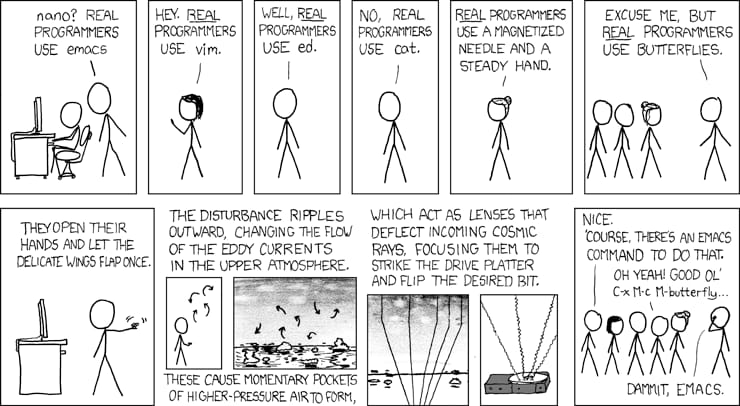
\includegraphics[width=0.85\textwidth, angle=34]{/home/buddhilw/PP/LaTeX/SEMEF-minicurso/Apresetacoes/g-img/meme-emacs.jpeg}
  
  \legend{Code Mesh, presentation ``Towers of Interpreters'', by Nada Amin}
\end{figure}



\section{Exercícios 1 - Lista 3}
\label{sec:orgb5a7f2d}
\section{Overleaf}
\label{sec:orgc748433}
\subsection{Texto com capa, tombo, e algum texto linguiça, uma imagem e uma tabela.}
\label{sec:org21f5099}
\begin{itemize}
\item \href{file:///home/buddhilw/PP/LaTeX/MC-LaTeX/LabEELw/LabEELw/MaterialMC/abnt\_modcanon/abntex2-modelo-include-comandos.tex}{Comentar a tabela e imagem} (documento autodocumentado do pacote ABNTeX2)
\item \href{TCC/TCC-en.tex}{TCC (Capa e tombo)}
\end{itemize}
\subsection{Apresentação beamer}
\label{sec:org12ec654}
\section{Alguns comentários}
\label{sec:orgc511f67}
\subsection{Apresentação Lupo}
\label{sec:org7d201cf}
\subsection{Fontes e materiais suplementares}
\label{sec:org0dfac84}
\subsection{Repositório criado para EEL-USP}
\label{sec:org9fec61f}
\end{document}